\chapter{Ergebnisse der Hyperparameter-Optimierung und des Trainings}
\section{Hyperparameter-Optimierung von \MiniDog}

In \autoref{fig:hyper-param} ist das Ergebnis der Hyperparameter-Optimierung von \MiniDog
dargestellt. Die optimalen Hyperparameter sind eine \texttt{Batch Size} von 2,
eine Stärke von 0.001 der \texttt{L2-Regularisierung} und die Verwendung
der Farbinformationen.

\begin{figure}
  \centering
  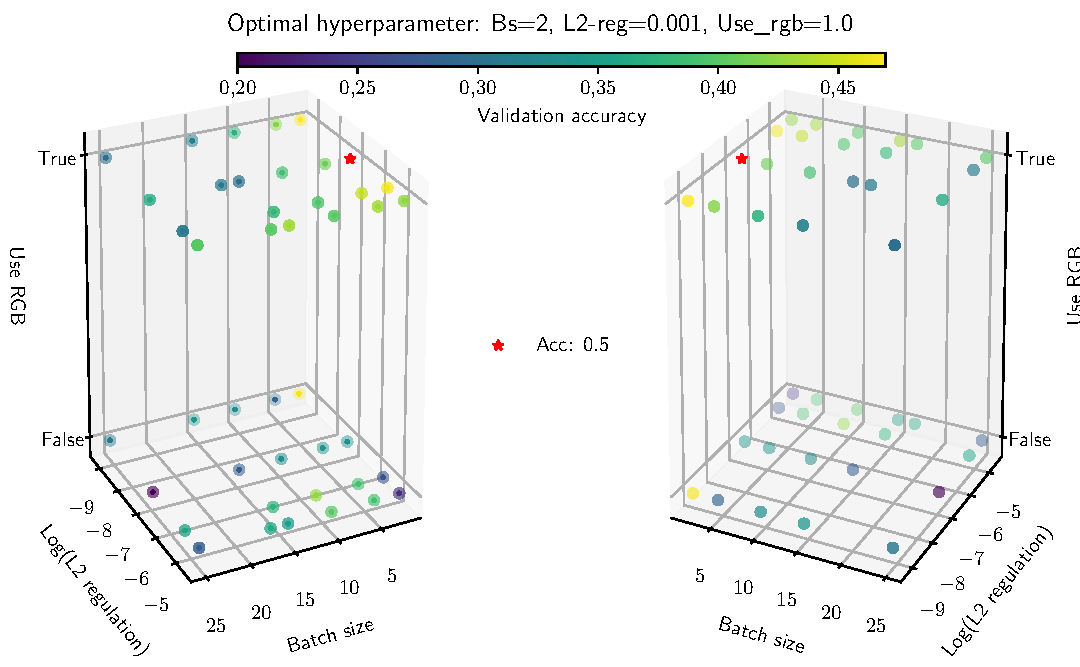
\includegraphics[width=\textwidth]{pics/ergebnisse/hyper_raum.pdf}
  \caption{Darstellung der Ergebnisse der Hyperparameter-Optimierung
  von \MiniDog. Die beste Kombination ist als Stern dargestellt und wurde auch
  für das Training verwendet.}
  \label{fig:hyper-param}
\end{figure}

Allgemein wird ersichtlich, dass in den meisten Fällen die Verwendung von Farbinformationen
zu einer höheren Validation Accuracy führt. Also kann eine der Fragen, ob die Verwendung
von Farbinformationen einen Vorteil in der Klassifikation bringt, mit Ja beantwortet werden.

\section{Verschiedene Bildgrößen beim  Training von \PreDog und \PreBig}

Wie bereits in \autoref{sec:größe-bilder} beschrieben, wurde für die beiden
Neuronalen Netze, die ein vortrainiertes Netz nutzen, alle Bilder 125x138
geresized. Dies erreichte eine Validation Accuracy von ungefähr \SI{60}{\percent}.
Falls die Bilder aber auf 224x224 geresized werden, dann steigt die Accuracy
auf ungefähr \SI{95}{\percent}. Da im kleinen Datensatz nur maximal 74 Bilder
kleiner sind als 224x224, die Validation Accuracy aber deutlich besser ist, wird diese Methode zum Training verwendet.
Loss und Accuracy Kurven sind im Anhang zu finden.

\section{\PreBig}

\begin{figure}
  \centering
  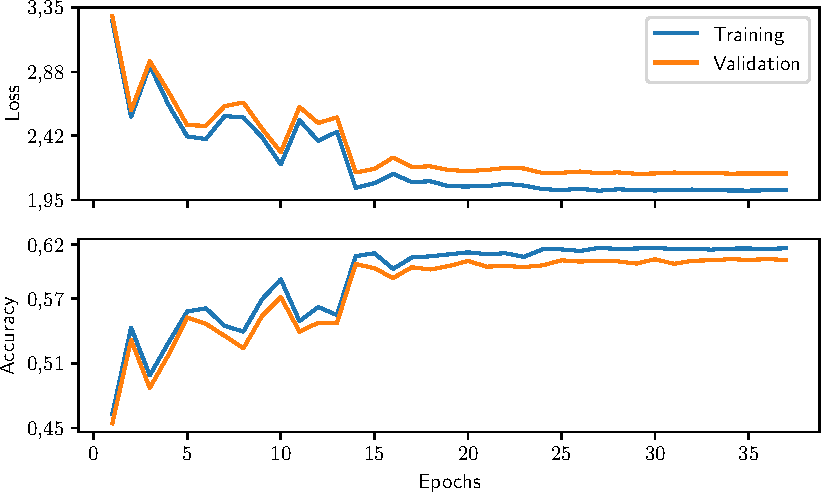
\includegraphics[width=\textwidth]{pics/ergebnisse/PreBigDogNN/history_epoch.pdf}
  \caption{Loss und Accuracy Kurven für \PreBig.}
  \label{fig:loss-acc-prebig}
\end{figure}

\begin{figure}
  \centering
  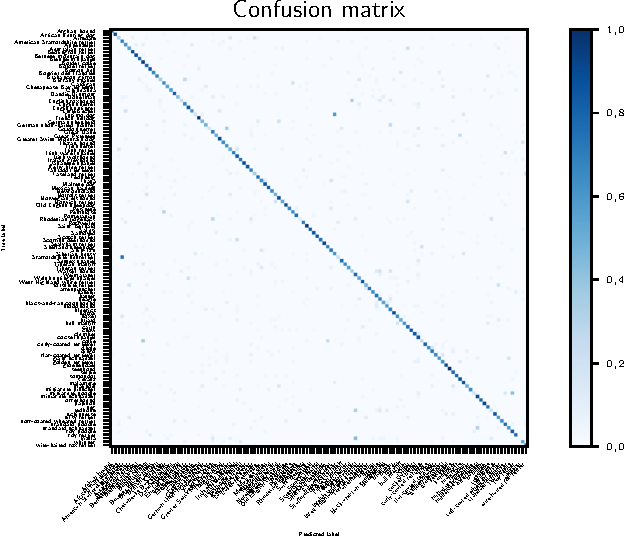
\includegraphics[width=\textwidth]{pics/ergebnisse/PreBigDogNN/confusion_matrix.pdf}
  \caption{Confusion Matrix für \PreBig.}
  \label{fig:confusion-prebig}
\end{figure}
